\section{Hidden Surprise}


    \begin{marginfigure}
\checkoddpage \ifoddpage \forcerectofloat \else \forceversofloat \fi
\centering
 \frame{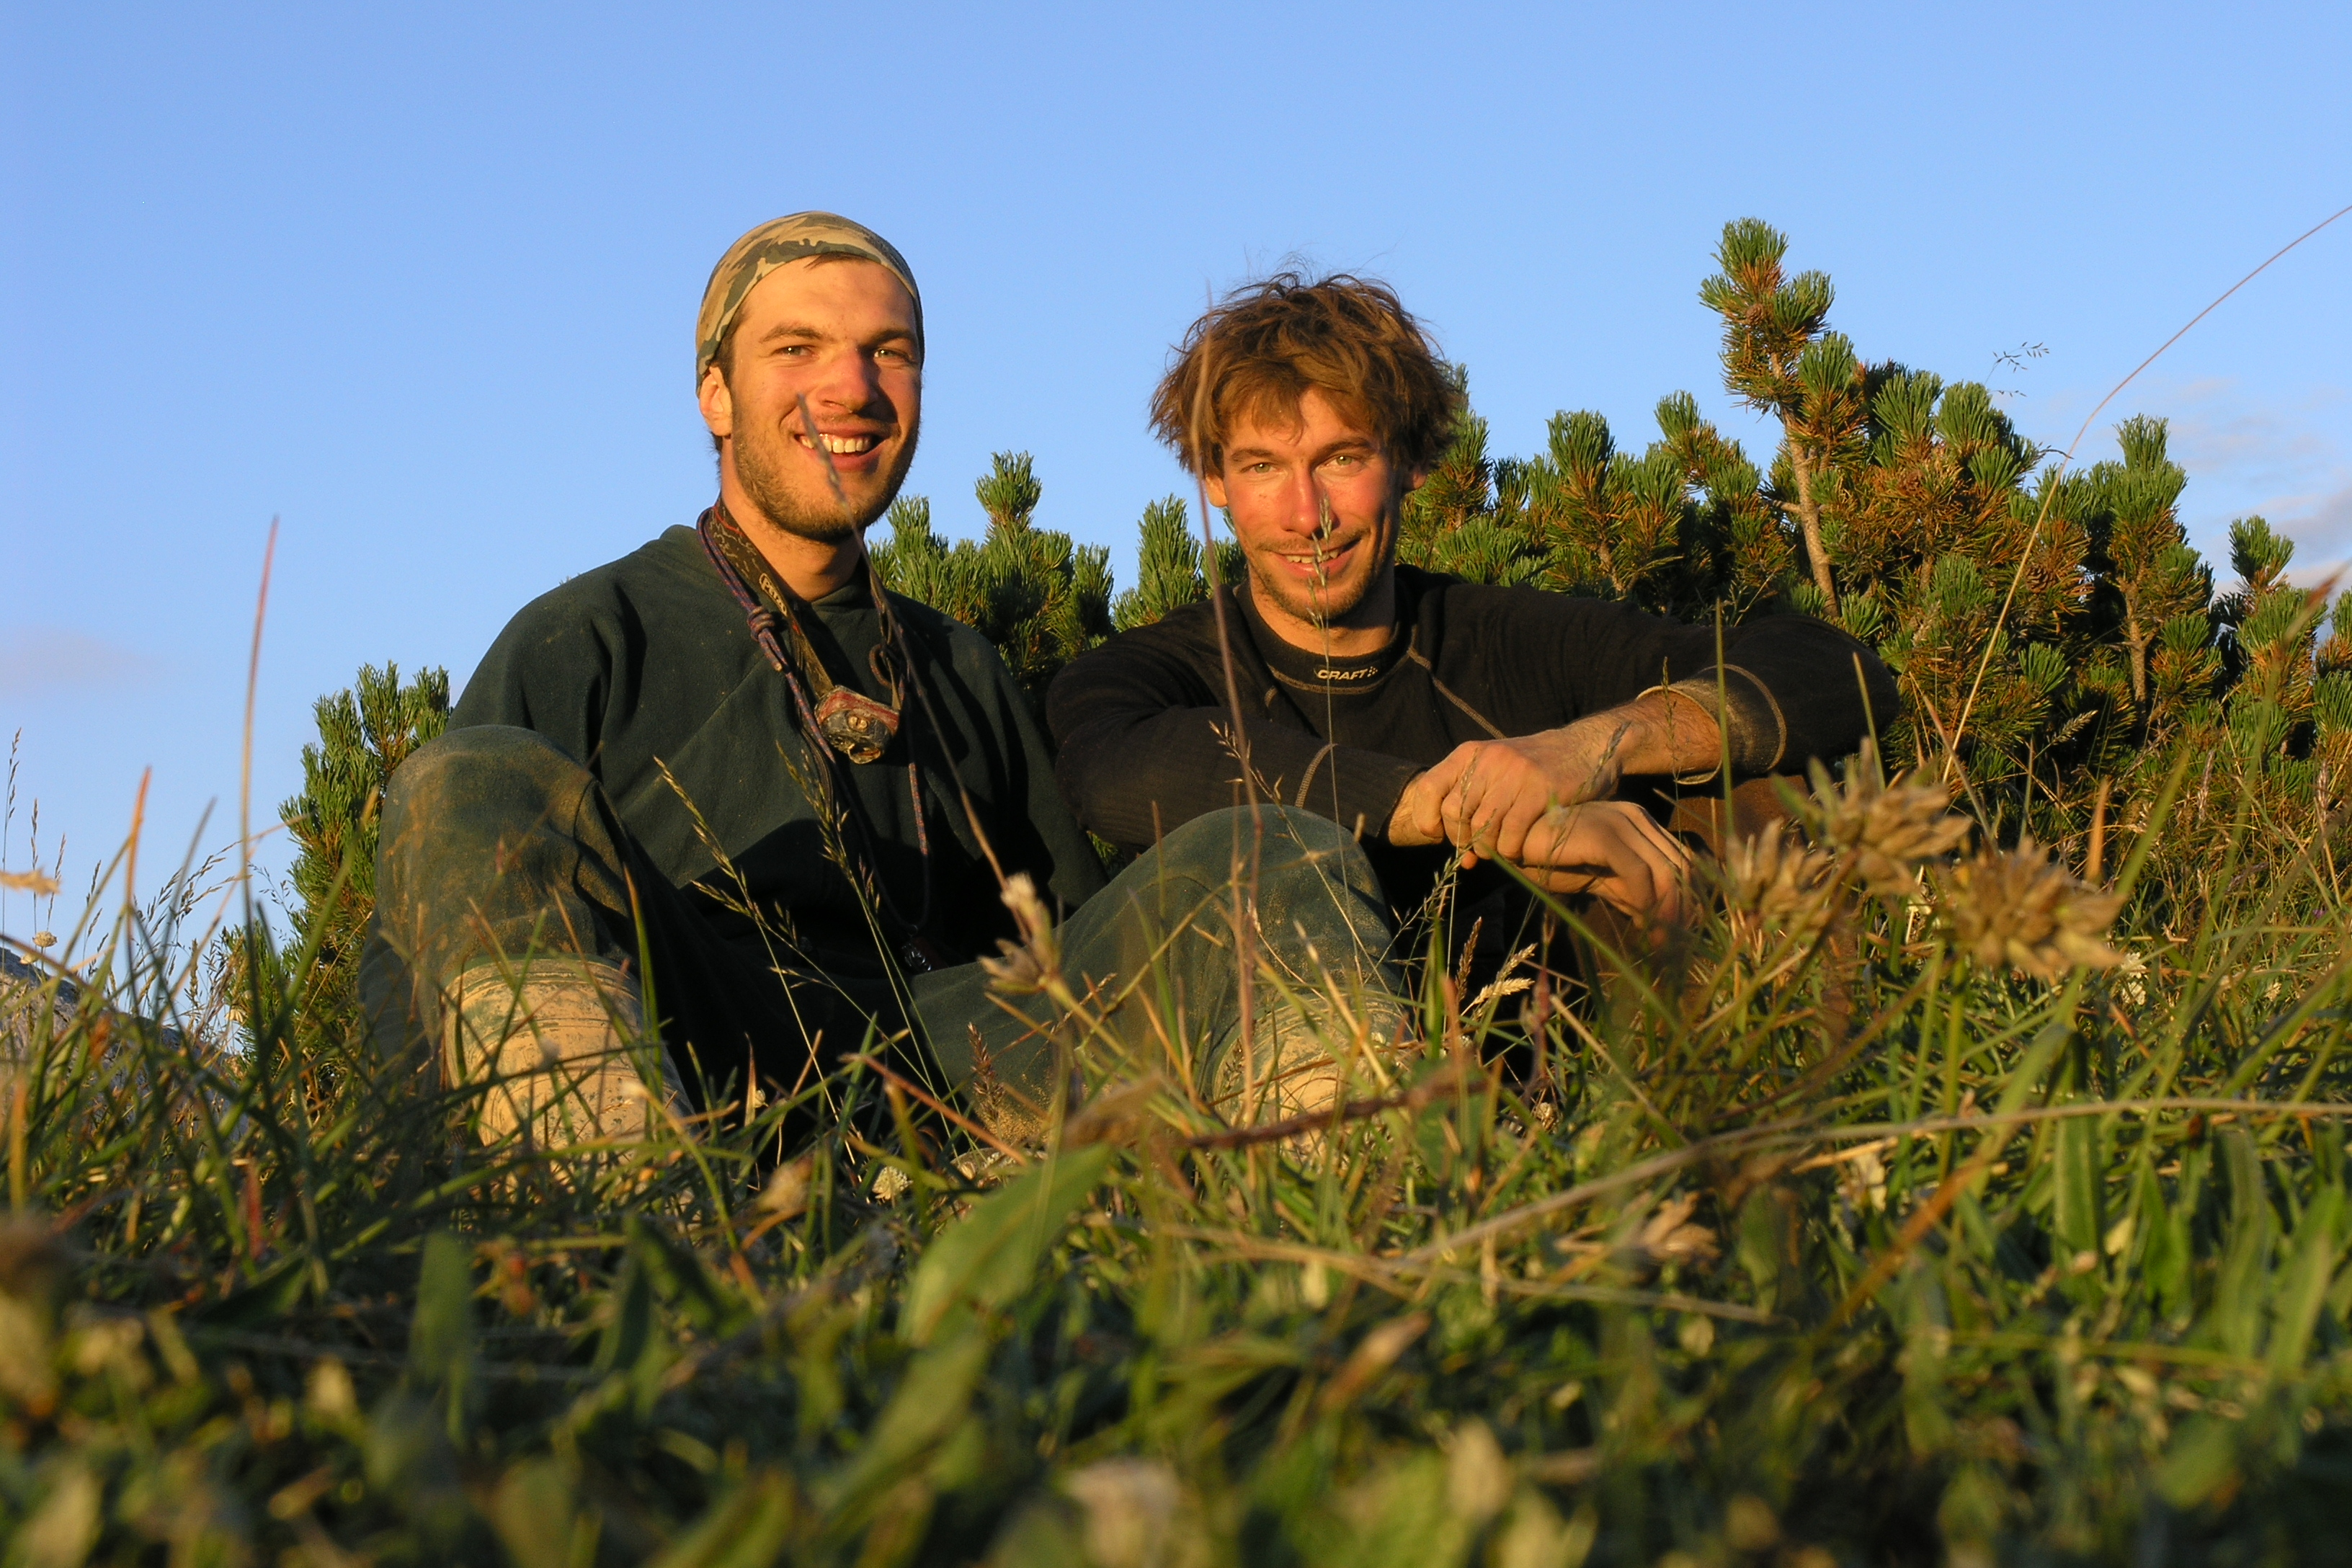
\includegraphics[width=\linewidth]{2010/palace/20100731-19-13-48 - Nikolas Kral - P7311788--orig.jpg}} 
 \caption{The Eastern European team of Slovakian Niko Kral and Hungarian Gergely Ambrus. \pic{Nikolas Kral}}
 \label{eastern european}
\end{marginfigure}

Well, the name \passage{Wonderland} does not really exist anymore, but back
then this was used for the horizontal level at the bottom of
\passage{Leopard}. Once finishing our triumphant trip with Andy, I was
eager to get back to continue the exploration of the many passages that
lay below. So, I paired up with Niko, to form a truly Eastern European
team, and went back to do what we had to do -- rig the drop at the end
of the \passage{Wonderland} passage!


\margininbox{Rolling Stones}{
     \begin{itemize}
    \item Gergely Ambrus
    \item Nikolas Kral
    \end{itemize}}{\explo}

Izi and Dan went to the other end, to find the continuation from the big
chamber (\passage{Albert Hall}). With Niko, we improved some of the rigging
that we did with Andy, and then dropped to the chamber with loose
boulders. Unfortunately, the rope that I used was new, and it shrunk
considerably later, so those rebelays have been too tight ever since.
Within the chamber, we climbed down to the obvious continuation, to find
to our horror an incredibly loose pitch within a pile of incredibly
loose boulders -- so we agreed that this was not the best option, if we
still want to do something else with our lives. Nevertheless, this
experience provided us with a good name -- \passage{Rolling Stones}! So,
there we were, in a nice big chamber, with a suicidal way onwards, and
we were not quite keen enough to continue that way\ldots{} We had a look
here and there, to no avail, and were about to turn back, when \bignote{Niko
climbed in between some rocks, and said in his usual slow manner --
``Heey maan}, maybe this is the right waay, nooo?'' And indeed it was!
Following the draught, we soon managed to open up a small passage, which
lead to a flat-out crawl, but after some 20 m it again popped in to
another chamber, quite nicely decorated. \passage{Hidden Surprise}! That
was the name we chose. The way on was obvious, and soon we emerged at
the top of a large black void space. This was a good point to turn back,
so we surveyed everything and showed it proudly to the happily emerging
pair of Izi and Dan. Then we returned to camp together, shared a nice
meal, talked about our stories, and had a nice evening, as usual at Camp
\passage{X-Ray}.

\margininbox{29.7 3am}{
Funny day train
steadily drifts towards night train. It is said that our natural day is
20-27 hours long\ldots{} \name{Gergely}}{\logbook}


\margininbox{Mudstone}{
     \begin{itemize}
    \item Gergely Ambrus
    \item Nikolas Kral
    \end{itemize}}{\explo}

Next day, we went back with Niko to the top of the pitch. Two ways were
at the offer: either down to the black, or across to the seemingly
obvious continuation of the phreatic tube. I was quite scared of going
down, so we chose the more safe option of doing the traverse. Niko put
in his first ever bolt at the Milka rock (which resembles a cow), and
then we slowly proceeded, given that the whole thing was done by hand
bolts. Finally I climbed up the slope on the other side (quite a scary
experience), and we were there at the start of kilometres of a wide,
walking phreatic passage! At least, we believed so. This expectation
proved to be immediately wrong, when after 15 m, we had to take off our
SRT kit in order to pass a squeeze. Never mind, we thought, the walking
passage is just on the other side! Well, not quite\ldots{} the ceiling
got lower and lower, and we really had to fight to advance about 50 m.
There, the passage became really low, so we decided to try to survey
back. It has been a gymnastic feast, not only small and low, but also
super uncomfortable because of the dry, fossilized mud formations that
filled the floor completely. Niko was super happy to be there -- the
afternoon was mostly passed by his constant ``Noo, maan''
moaning\ldots{} The mud formations are indeed very nice, maybe they
should be scientifically investigated. Anyway, they gave the place a
name -- \passage{Mudstone Squeeze} and \passage{Mudstone Traverse} were what we
surveyed that day. To this date, nobody has been back to \passage{Mudstone
squeeze} -- although \bignote{it is quite a place to go, if you happen to have
some free time and want to exercise your squeezing and crawling skills}!
:)

\name{Gergely Ambrus}




\section{Palace of King Minos, Queens Bed Chamber, Minotaur Rift and Ouroboros}


Last year we manage to connect \passage{Captain Kangaroo} with lower parts of \passage{Vrtnarija} (\passage{Friendship Gallery}), so I could not wait to go caving again, especially to first descent the whole \passage{Pico}.

Dan and I decided to go camping in \passage{X-Ray}, re-established after many years.

We were on the night train. So the plan was to go caving late at night,
reach the camp in the morning and then go straight to bed. When we
reached the camp we find a note, asking if we could wait a bit longer,
because the other team return late. We decided to go and check out the
newly discovered parts and maybe find some leads for tomorrow. When we
return to \passage{X-Ray} we meet our tent mates Gergely and Niko, who just
return from their caving trip. We prepared some food, change to dry
clothes and went into sleeping bags, while others started preparing for
caving. It was funny to watch how they were not happy to put on wet
caving clothes.

\name{Izi Možir}



\begin{marginfigure}
\checkoddpage \ifoddpage \forcerectofloat \else \forceversofloat \fi
\centering
 \frame{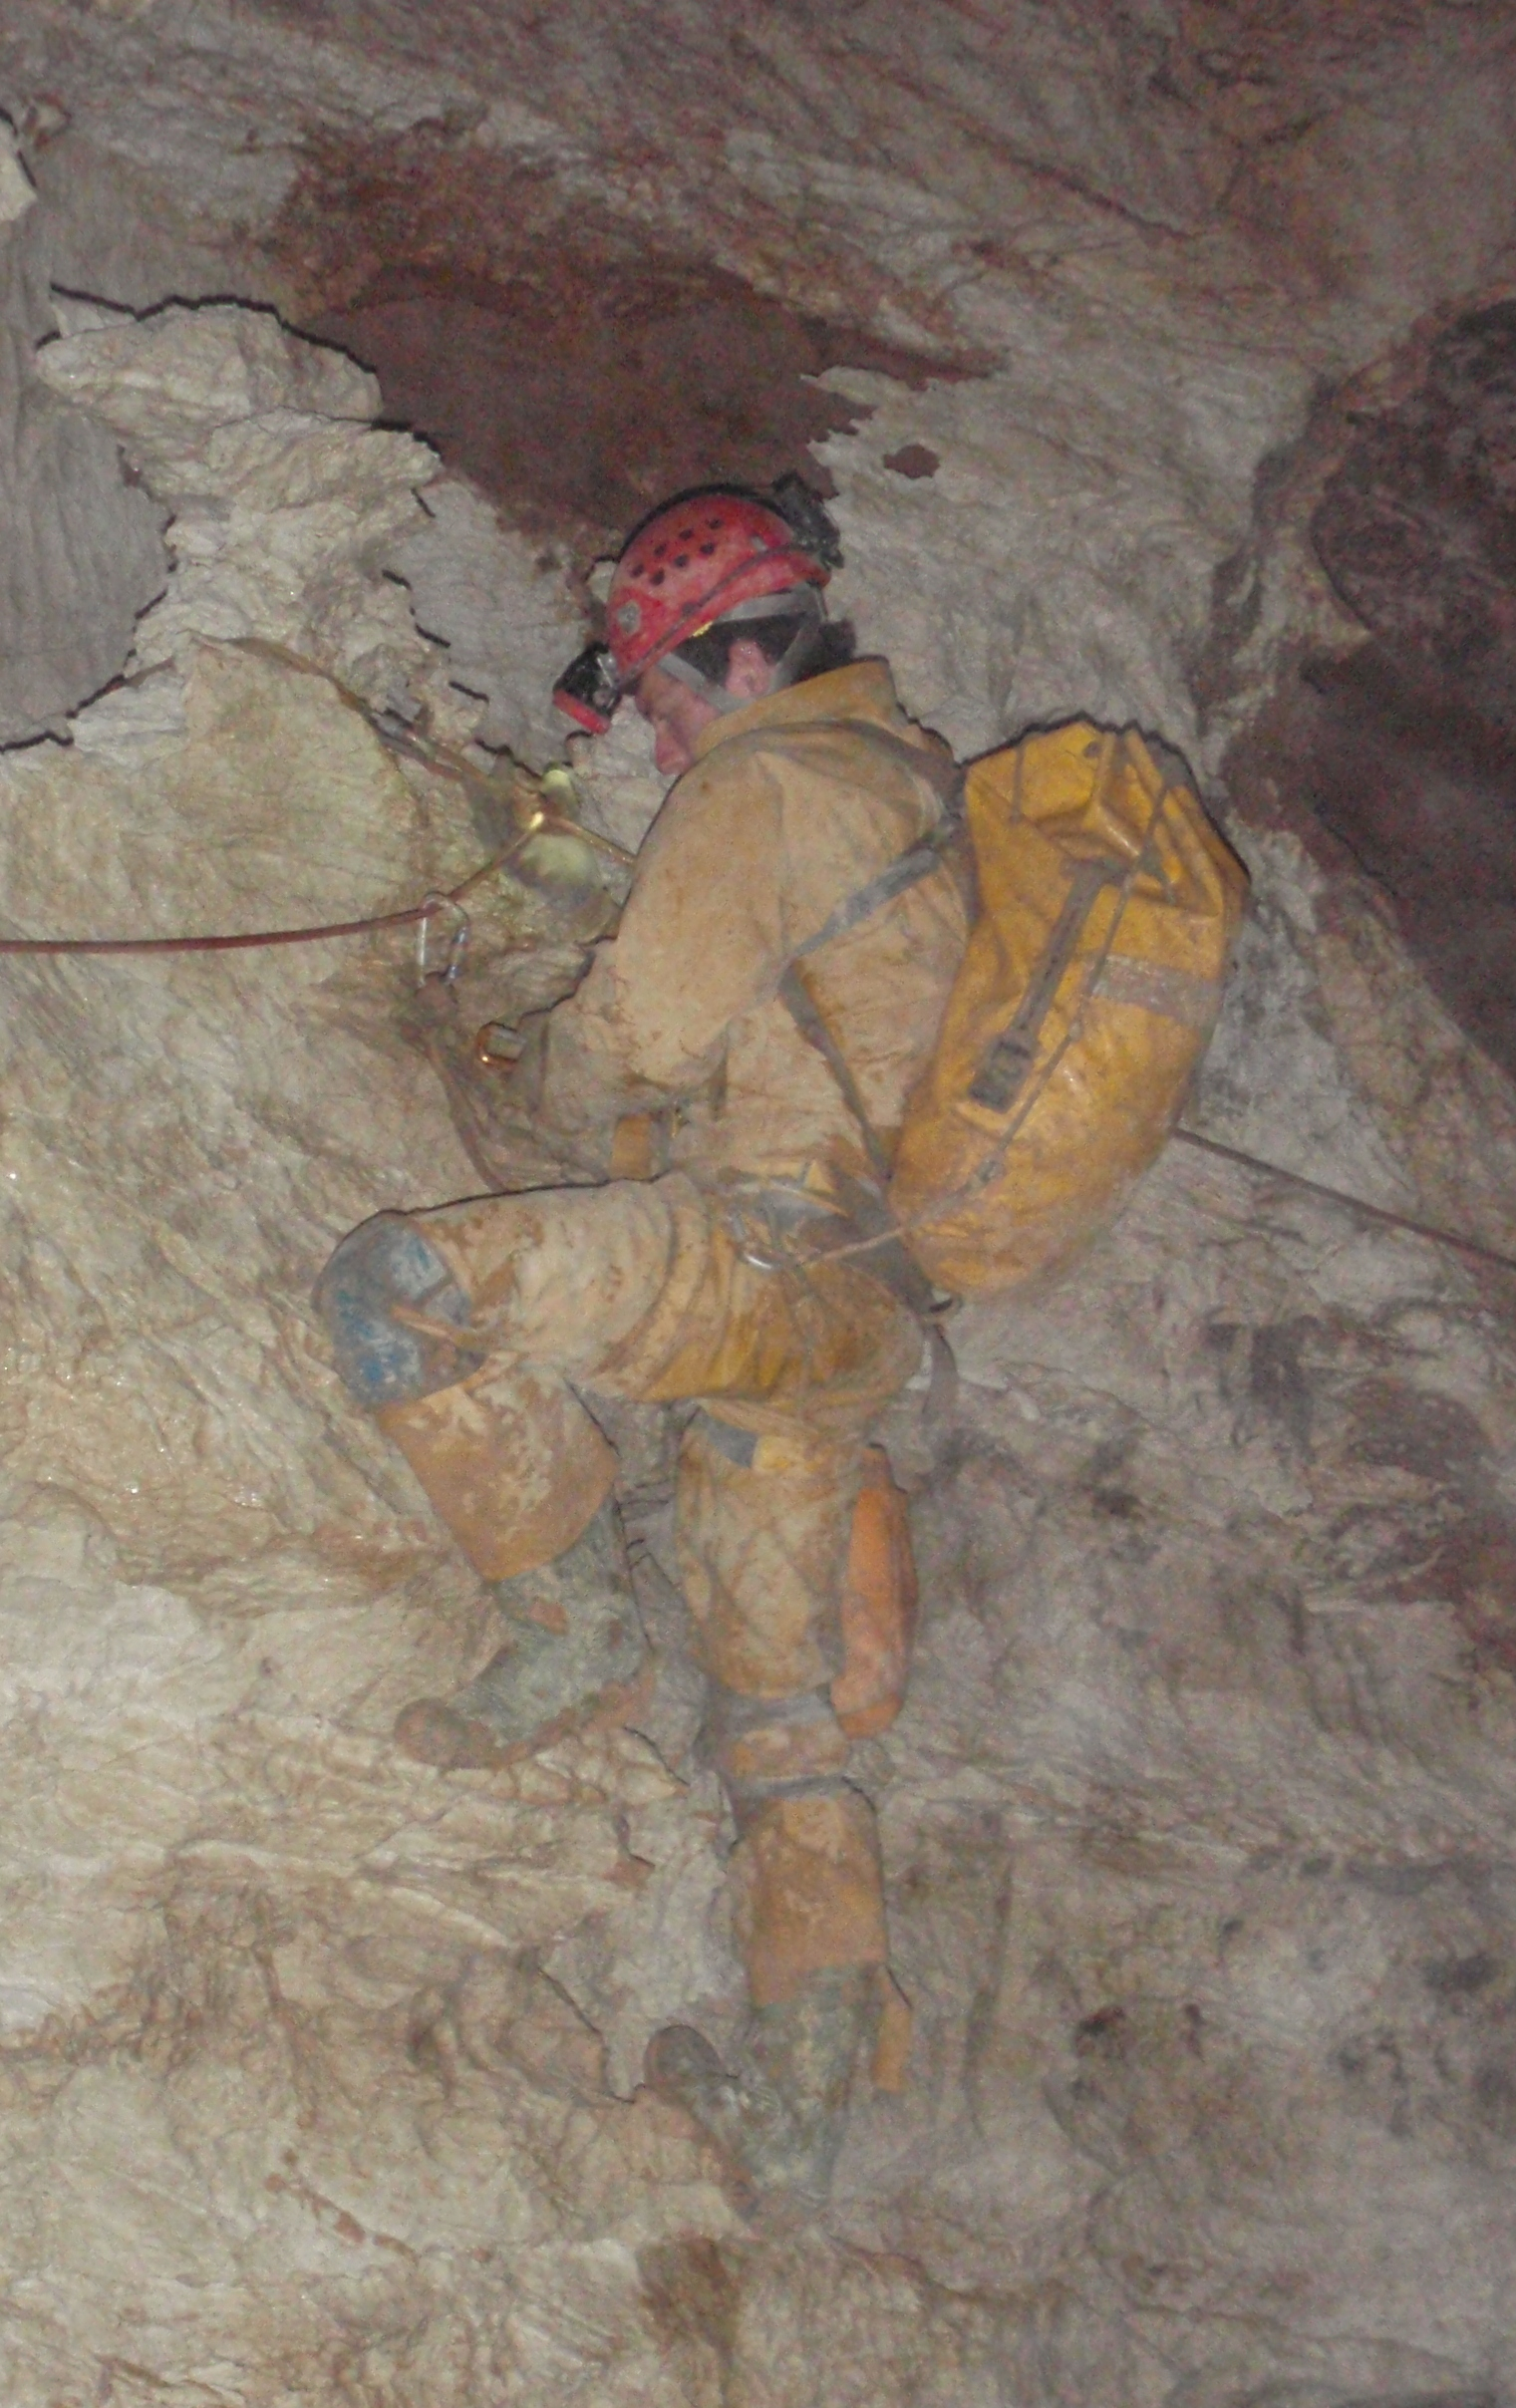
\includegraphics[width=\linewidth]{2010/palace/20100728-20-44-16 - Iztok Mozir - P7284645 - first traverse on Prince Consort Road--snip--orig.jpg}} 
 \caption{Traversing in \protect\passage{Prince Consort Road}. \pic{Iztok Možir}}
 \label{prince consort traverse}
\end{marginfigure}

\begin{figure*}[t!]
      \checkoddpage \ifoddpage \forcerectofloat \else \forceversofloat \fi
      \centering
    \begin{subfigure}[t]{\textwidth}
    \centering
        \frame{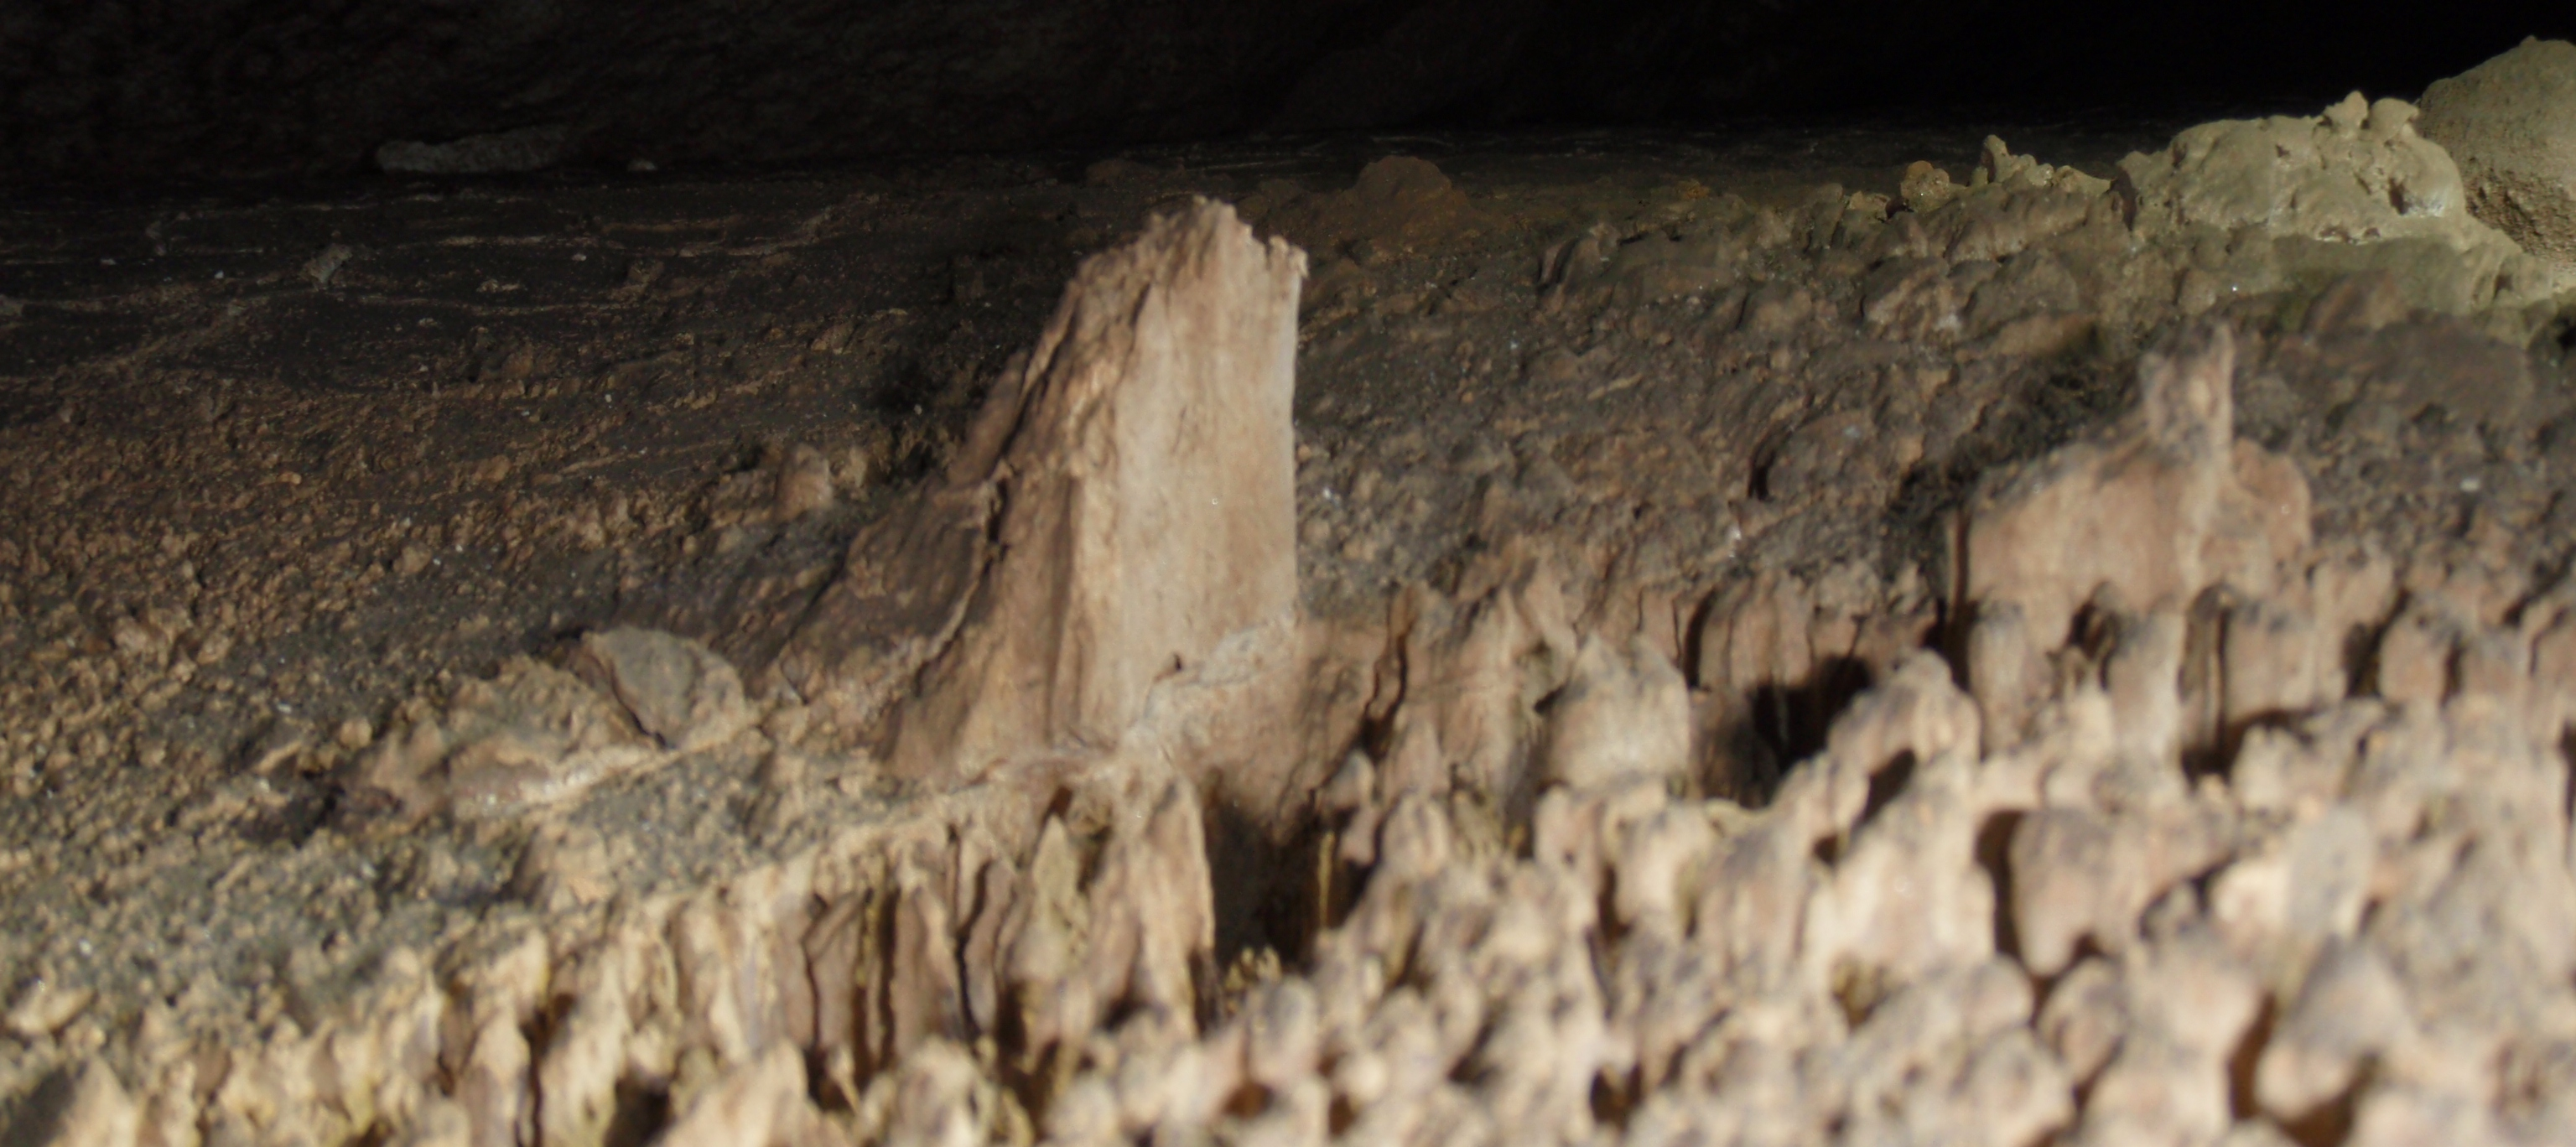
\includegraphics[width=\linewidth]{2010/palace/20100803-06-05-22 - Iztok Mozir - P8034784 - Palace of King Minos and Prince Consort Road-thin--orig.jpg}} 
        \caption{} \label{mud palace}
    \end{subfigure}
    
          \vspace{0.3cm}
          
    \begin{subfigure}[t]{0.555\textwidth}
        \centering
        \frame{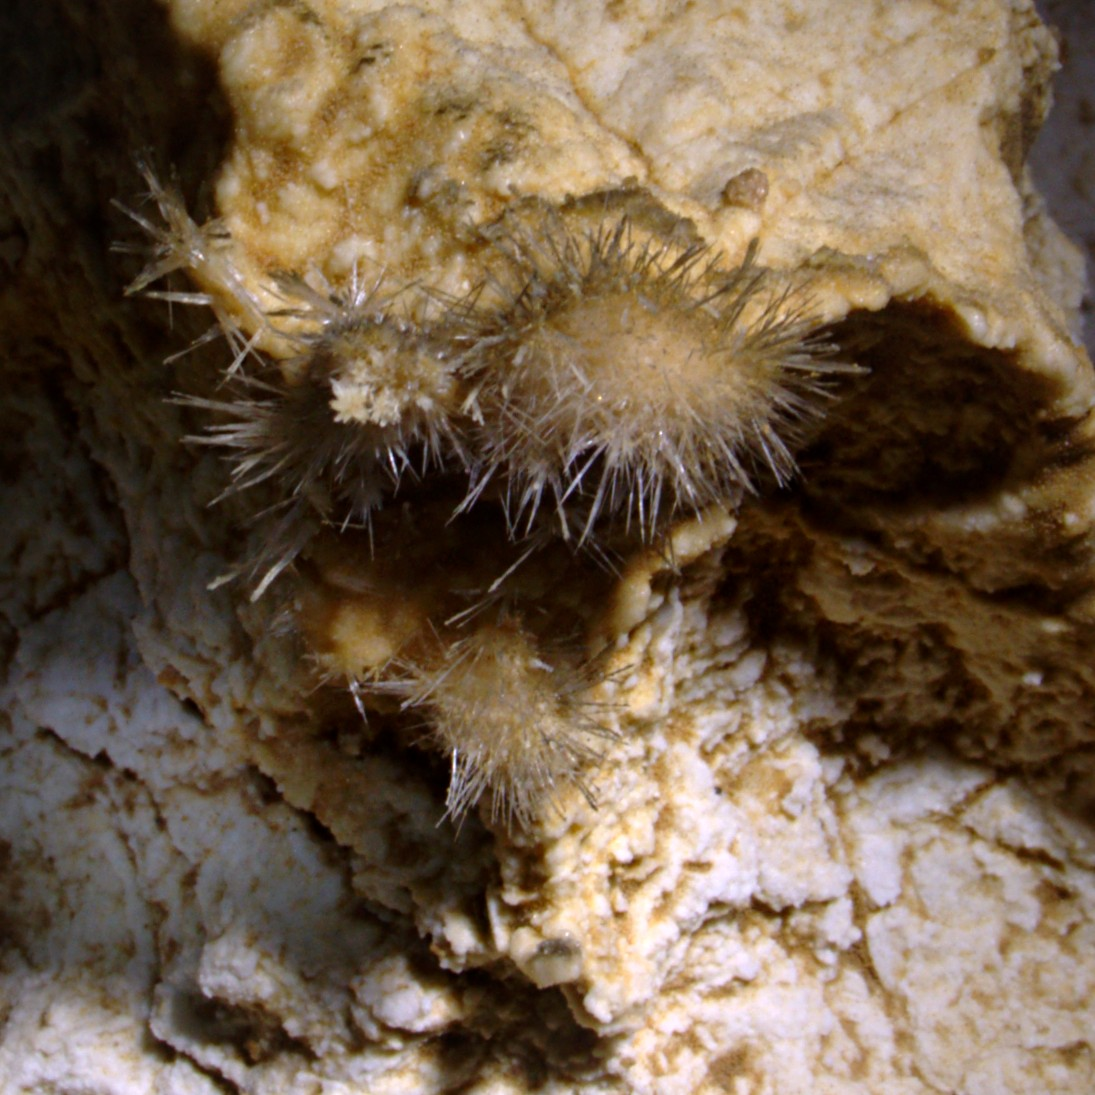
\includegraphics[width=\linewidth]{2010/palace/20100731-19-02-10-Jarvist Frost-Canon G5-CRW_0327-crop-Crystals at Start of Palace of King Minos--square--orig.jpg}} 
        \caption{} \label{square crystals}
    \end{subfigure}
    \hfill
    \begin{subfigure}[t]{0.418\textwidth}
        \centering
        \frame{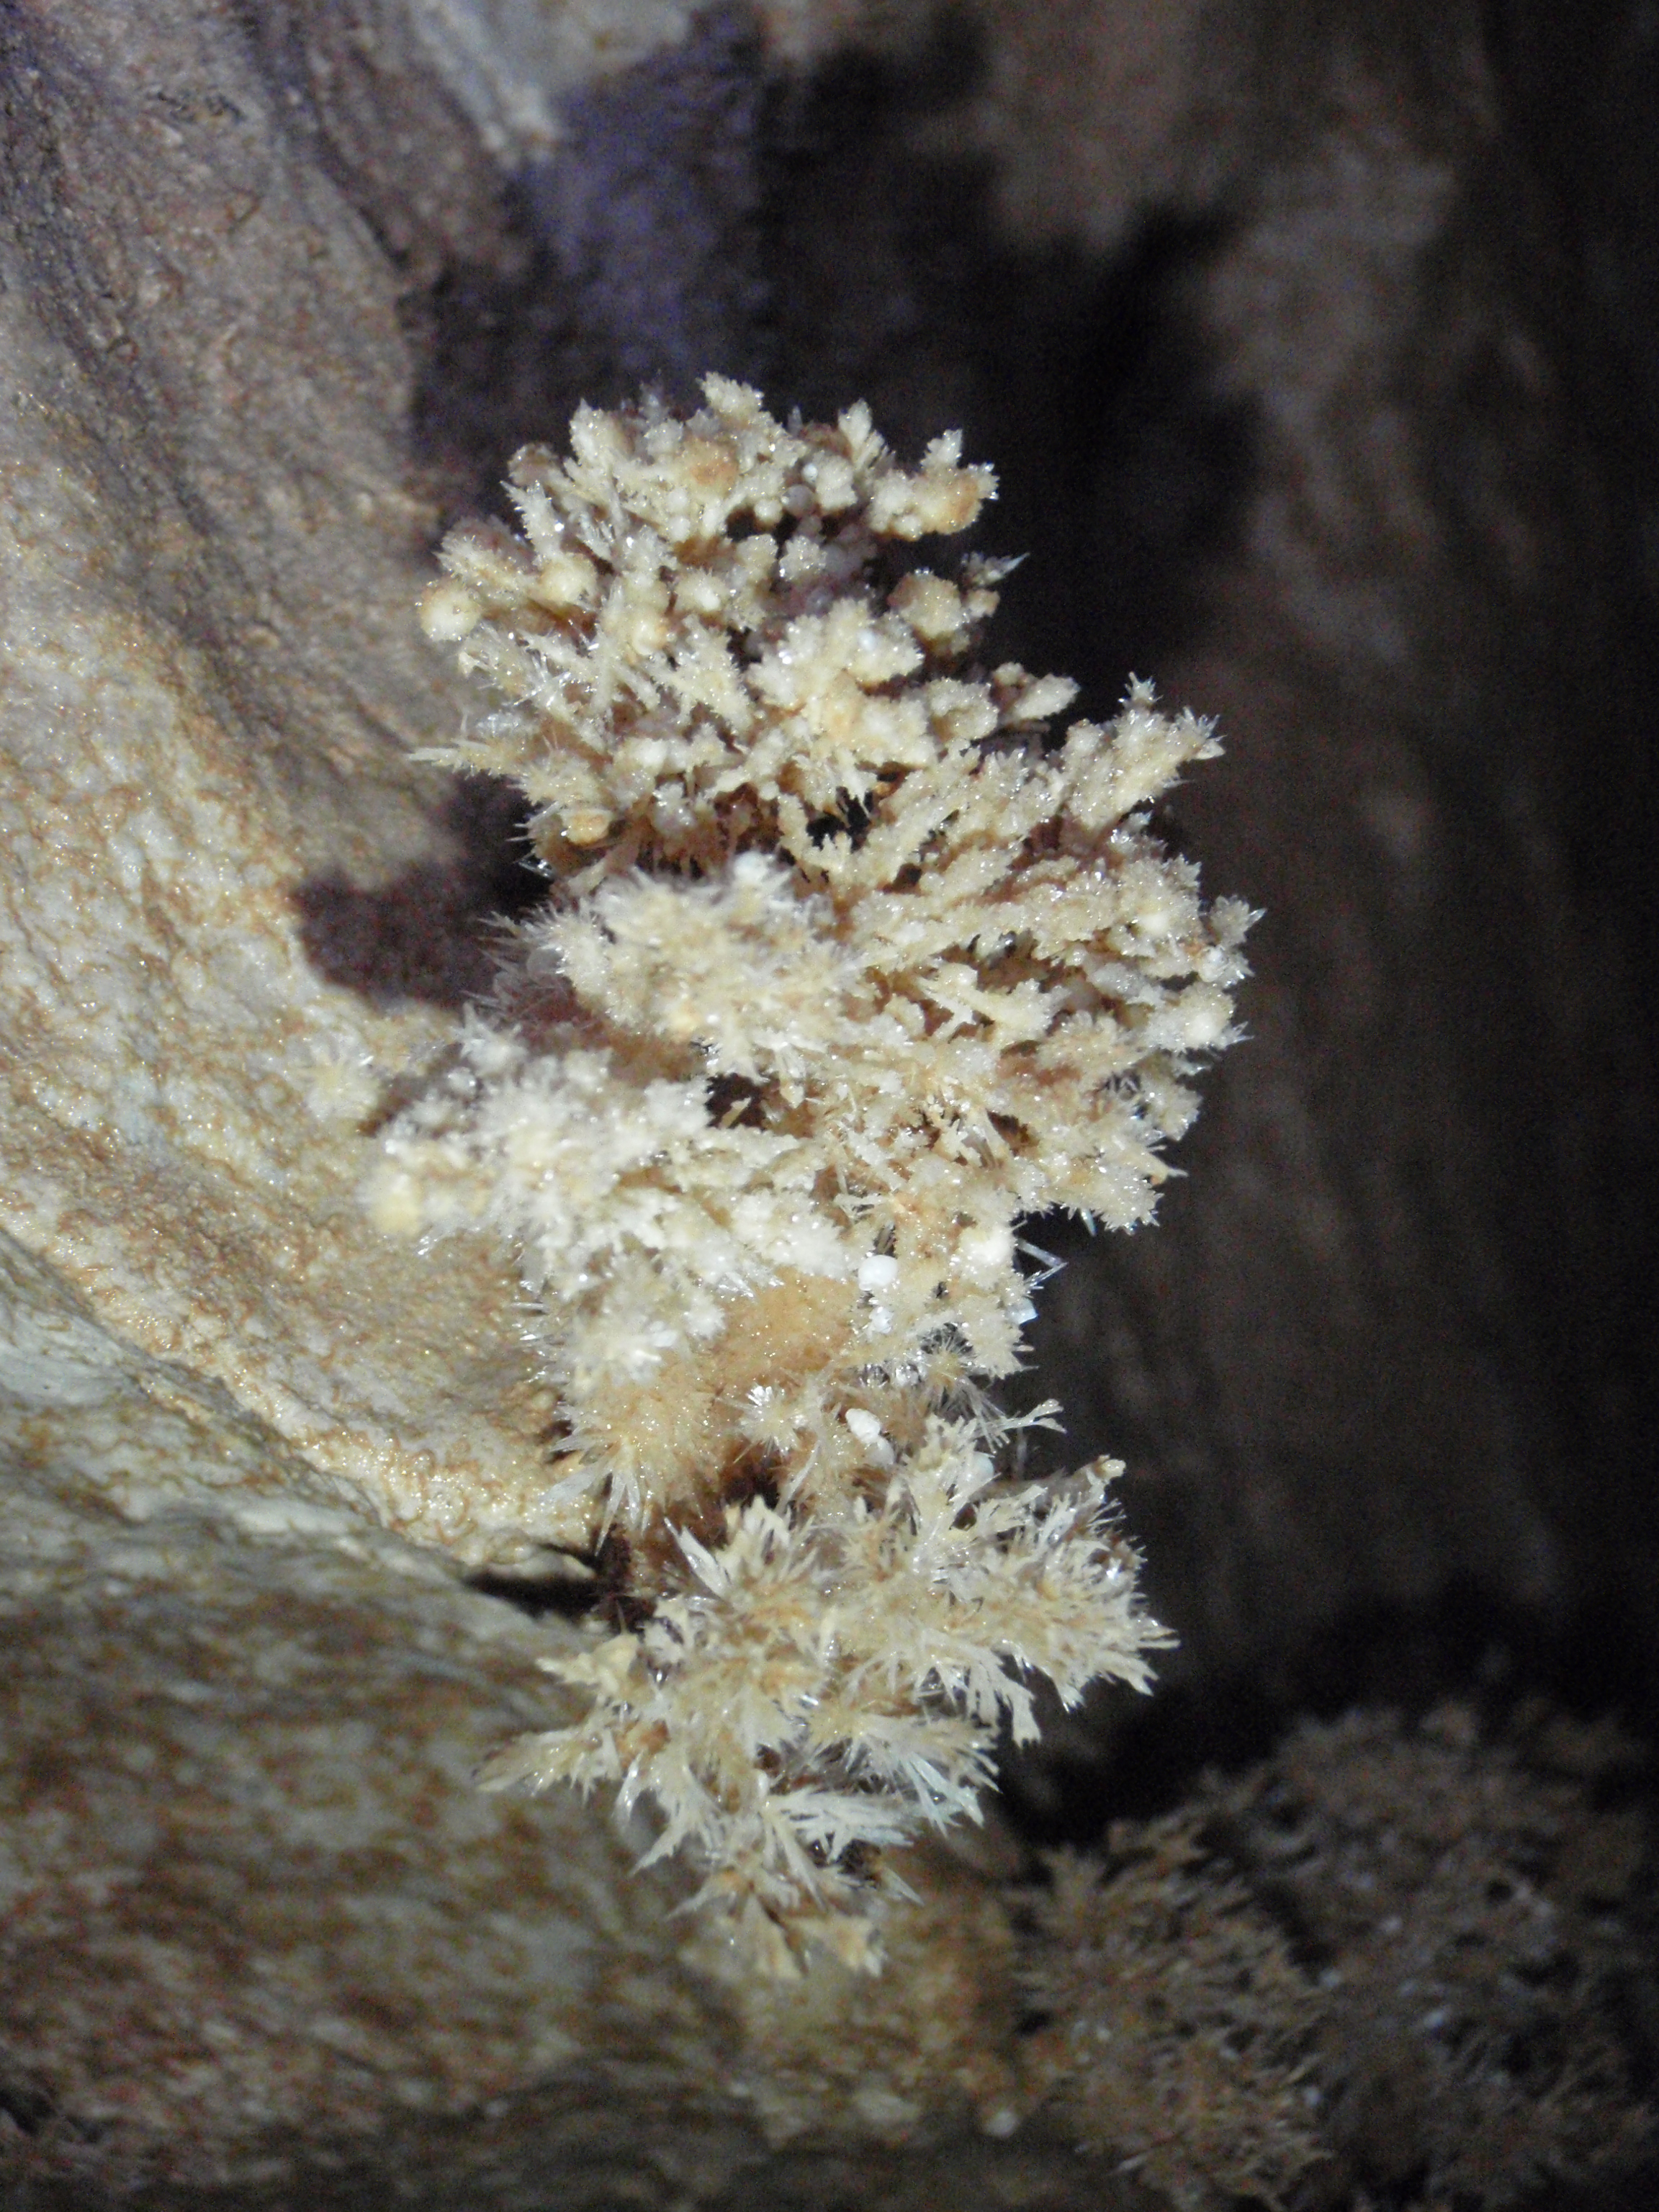
\includegraphics[width=\linewidth]{2010/palace/20100803-05-52-27 - Iztok Mozir - P8034776 - Palace of King Minos and Prince Consort Road--orig.jpg}} 
        \caption{} \label{crystal formation}
    \end{subfigure}

    \caption{Formations in the \protect\passage{Palace of King Minos}.
    \textit{(a)} Mud formations. \pic{Iztok Možir}
    \textit{(b)} Crystals at the start of the \protect\passage{Palace of King Minos}. \pic{Jarvist Frost}
    \textit{(c)} More crystals. \pic{Iztok Možir}}
\end{figure*}



We were woken up by Jarv (ed:James) and Jan who just return from their pushing trip. While cursing wet clothes we discussed what they had found and what was worth visiting and pushing. Soon we took off and separated on the bottom of \passage{Cheetah}.


Gergely and Niko went down \passage{Wonderland}, Dan and I went to
\passage{Prince Consort Road}. Road lead us to \passage{Albert hall} where not
long ago Jarv and Jan(ed:NOT JAN?!) were pushing \passage{Serpentine}. We decided to push some
new leads, so we climbed higher in this chamber and from there we saw a
big gallery. To reach this gallery we needed to climb about 6 m high.
Dan gave me a push up and I was able to reach the top. There I secured
the rope around the bolder and Dan joined me. From there we made a
traverse and then entered the gallery. Already on the entrance we
noticed something amazing. The ceiling was covered with white crystals,
that we never accounted[sic] before. That meant this is an old phreatic
gallery and we were so lucky to be the first one to discover it. Also
the soil on the ground was brown on top and once we stepped on it, it
was white underneath. Our first steps left white trails of footsteps
behind, truly amazing. We were really careful with our steps, as we did
not want to make to much damage. We mainly stick to the main passage and
there were no pitches or tight squeezes, perfect for exploring. On the
end of this gallery we were stopped by an aven. We could not climb it,
so we decided to return and start surveying back. On the way back we
took another side passage which lead us back to \passage{Albert hall}.
Because we made a loop and the whole place look like a maze, we name it
\passage{Palace of King Minos}, the side passage was named \passage{Ouroboros}, cuz it was a
loop to \passage{Albert hall} and also we named the big rift \passage{Minotaur}. We
left one side passage for next time, because we were already tired.
Surveying this gallery was a pure joy. Long distances between stations,
minimum of 10 m. Both of us were extremely happy with our discovery and
so we return to \passage{X-Ray} for well deserved rest. In the camp we meet
the other team and also they find some new meters. We exchange our trip
experience and fall asleep.

\name{Izi Možir}


\margininbox{31.7 Sat (morning?)}{Went to check out passages discovered day
ago by Dan and Izi. Very Beautiful! Looks like it snowed there but
upside down, the crystal formations are crazy, definitely have to come
down with camera for photo trip. Jan and James stayed down here as well,
and day and night train kind of blended together. \name{Nick}}{\logbook}



Back at the camp, we heard the great news: Izi and Dan just found 600 m
of passage at the \passage{Palace of King Minos}! We were about to exit the cave
the next morning, but there apparently had been a great storm, making
\passage{Zimmer} impassable for a good 20 hours. So we got the opportunity
to have a tourist trip to \passage{Palace of King Minos}, and we did very well to use
it - an absolutely amazing bit of cave! After another night at camp, we
finally started to the surface after 4 days underground, but we were
certain to return to the plethora of exciting leads\ldots{}

\name{Gergely Ambrus}


When we woke up, we were surprised by roaring in \passage{Zimmer}. During
the day it was raining outside, therefore a lot of water was purring
down \passage{Zimmer}. Dan and I still have one more night at a camp, but
because Niko and Gergely were not feeling to go out in these conditions,
we volunteered to do it. Beside, someone had to cancel their call out.
So we eat something and start going up to the surface. I was first
heading out, but before I fully attached myself on the rope in
\passage{Zimmer}, I was already all wet. I told Dan that I will not wait
for him and because we both know the way out, we will see each other on
the surface.

\tweet{8:54AM Jul 31st, 2010}{Couple braved the wet pitches at the ebb of the flood pulse to bring us all ok from camp, and 550m of horiz survey, PALACE OF KING MINAS!}

I was going for about an hour, stopped, roll 2 cigarettes,
smoke one, and leave one for Dan and then continue out. Below
\passage{Pico}, I repeated the same procedure, so at that time Dan catches
me up and we continued together. Above \passage{Pico} it was less water so
that meant that the rain has stop. We reached the surface in 3 and half
hours. In the bivy we entered the data and we were so happy when we
heard that we surveyed more than 500 m, especially how easy was to do
it.

\name{Izi Možir}











\newpage
\begin{pagefigure}
\checkoddpage \ifoddpage \forcerectofloat \else \forceversofloat \fi
\frame{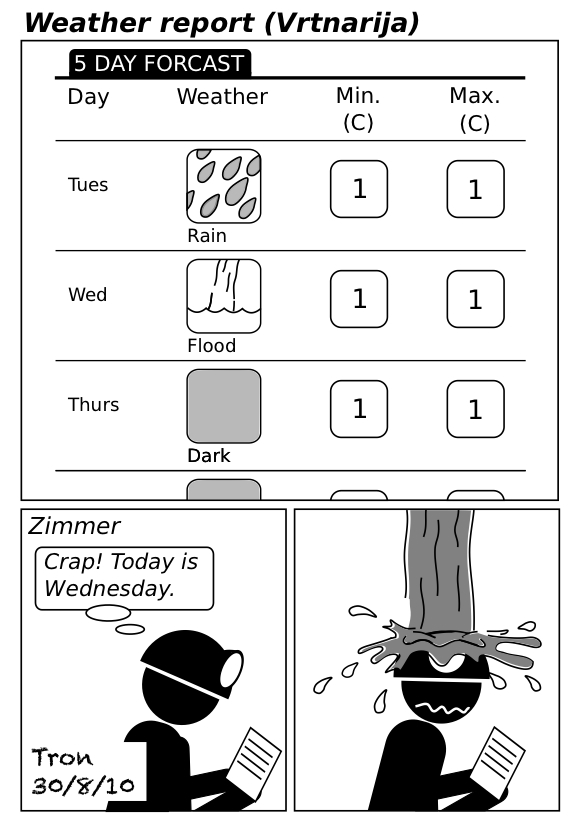
\includegraphics[width=\linewidth]{2010/palace/Tharatorn Supasiti - March 2012 - vrtnirija-weather--orig.jpg}}
\caption{And now, the weather\ldots{} ah, rain again, is it? \pen{Tharatorn Supasiti}} \label{Zimmer cartoon}
\end{pagefigure}
